\chapter{研究背景}
\label{chap:haikei}

本章では手書きメモ・イラストを扱う既存のシステムの現状と、その問題点を整理する。

\newpage

%\section{手書きのメモ・イラスト}
%手書きによるメモやイラストは情報を記録・表現する手法として広く普及している。
%筆記具と紙さえあればすぐに記録でき、また美麗な作品を描くことを目的としなければ、特別な技量も要求されないためである。
%計算機の登場によりテキスト編集支援機能が充実したため、文章のみで完結する内容であれば手書きではなくテキストとして記録するように置き換わったが、
%アイデアのような文章のみでは表現しづらい構造を持った概念を表現する場合は文字と図を自在に混合させて配置できる手書きメモの方が適している。
%また、テキストによってメモをとる場合はキーボードのような専用のハードウェアや、それらを使いこなすタッチタイピング等の技量が必要であるという問題点があるが、
%手書きの場合は紙やペン等の筆記具が扱えれば良いため、ハードウェアや技能を必要とするテキスト入力と比較してより多くの人々が利用できる手段であると言える。
%%そもそもの手書きメモの存在意義を説明する
%%(それが現代でもテキストには完全に置き換えられないことを示す)
%%そしてペンによるインターフェースを備えたデバイスが普及したことに手書きメモもテキスト

\section{手書きメモ・イラスト}
手書きによるメモやイラストは情報を記録・表現する手法として広く普及している。
例えば物体のスケッチ等の視覚的な情報やアイデアのような文章のみでは表現しづらい構造を持つ概念
等を表現する場合は、文字と図を自在に混合させることができる手書きメモの方が、テキストのみを使用したメモよりも柔軟に記録できる。
さらに手書きメモの作成にあたってはペンさえ握れれば良く、タッチタイピング等の特別なスキルも必要としないためテキスト入力と比較して
より多くの人々にとって利用しやすい表現手段であると言える。

またiPad(図\ref{fig:ipad})やSurface(図\ref{fig:surface})等のペンによるインターフェースを備えたタブレットデバイスが普及した現在では、
テキストと同じく計算機上でも手書きのメモやイラストが描かれるように変化した。
これにより手書きのメモやイラストを描く際にUndo/Redoやコピー&ペースト等の編集支援機能を利用できるようになり、利便性が向上した。
一方でテキストと異なり手書きのデータそのものを検索することができないため、作成した手書きメモの運用については不便な点が存在する。

\begin{figure}[htbp] \begin{minipage}{0.5\hsize}
                         \begin{center} \fbox {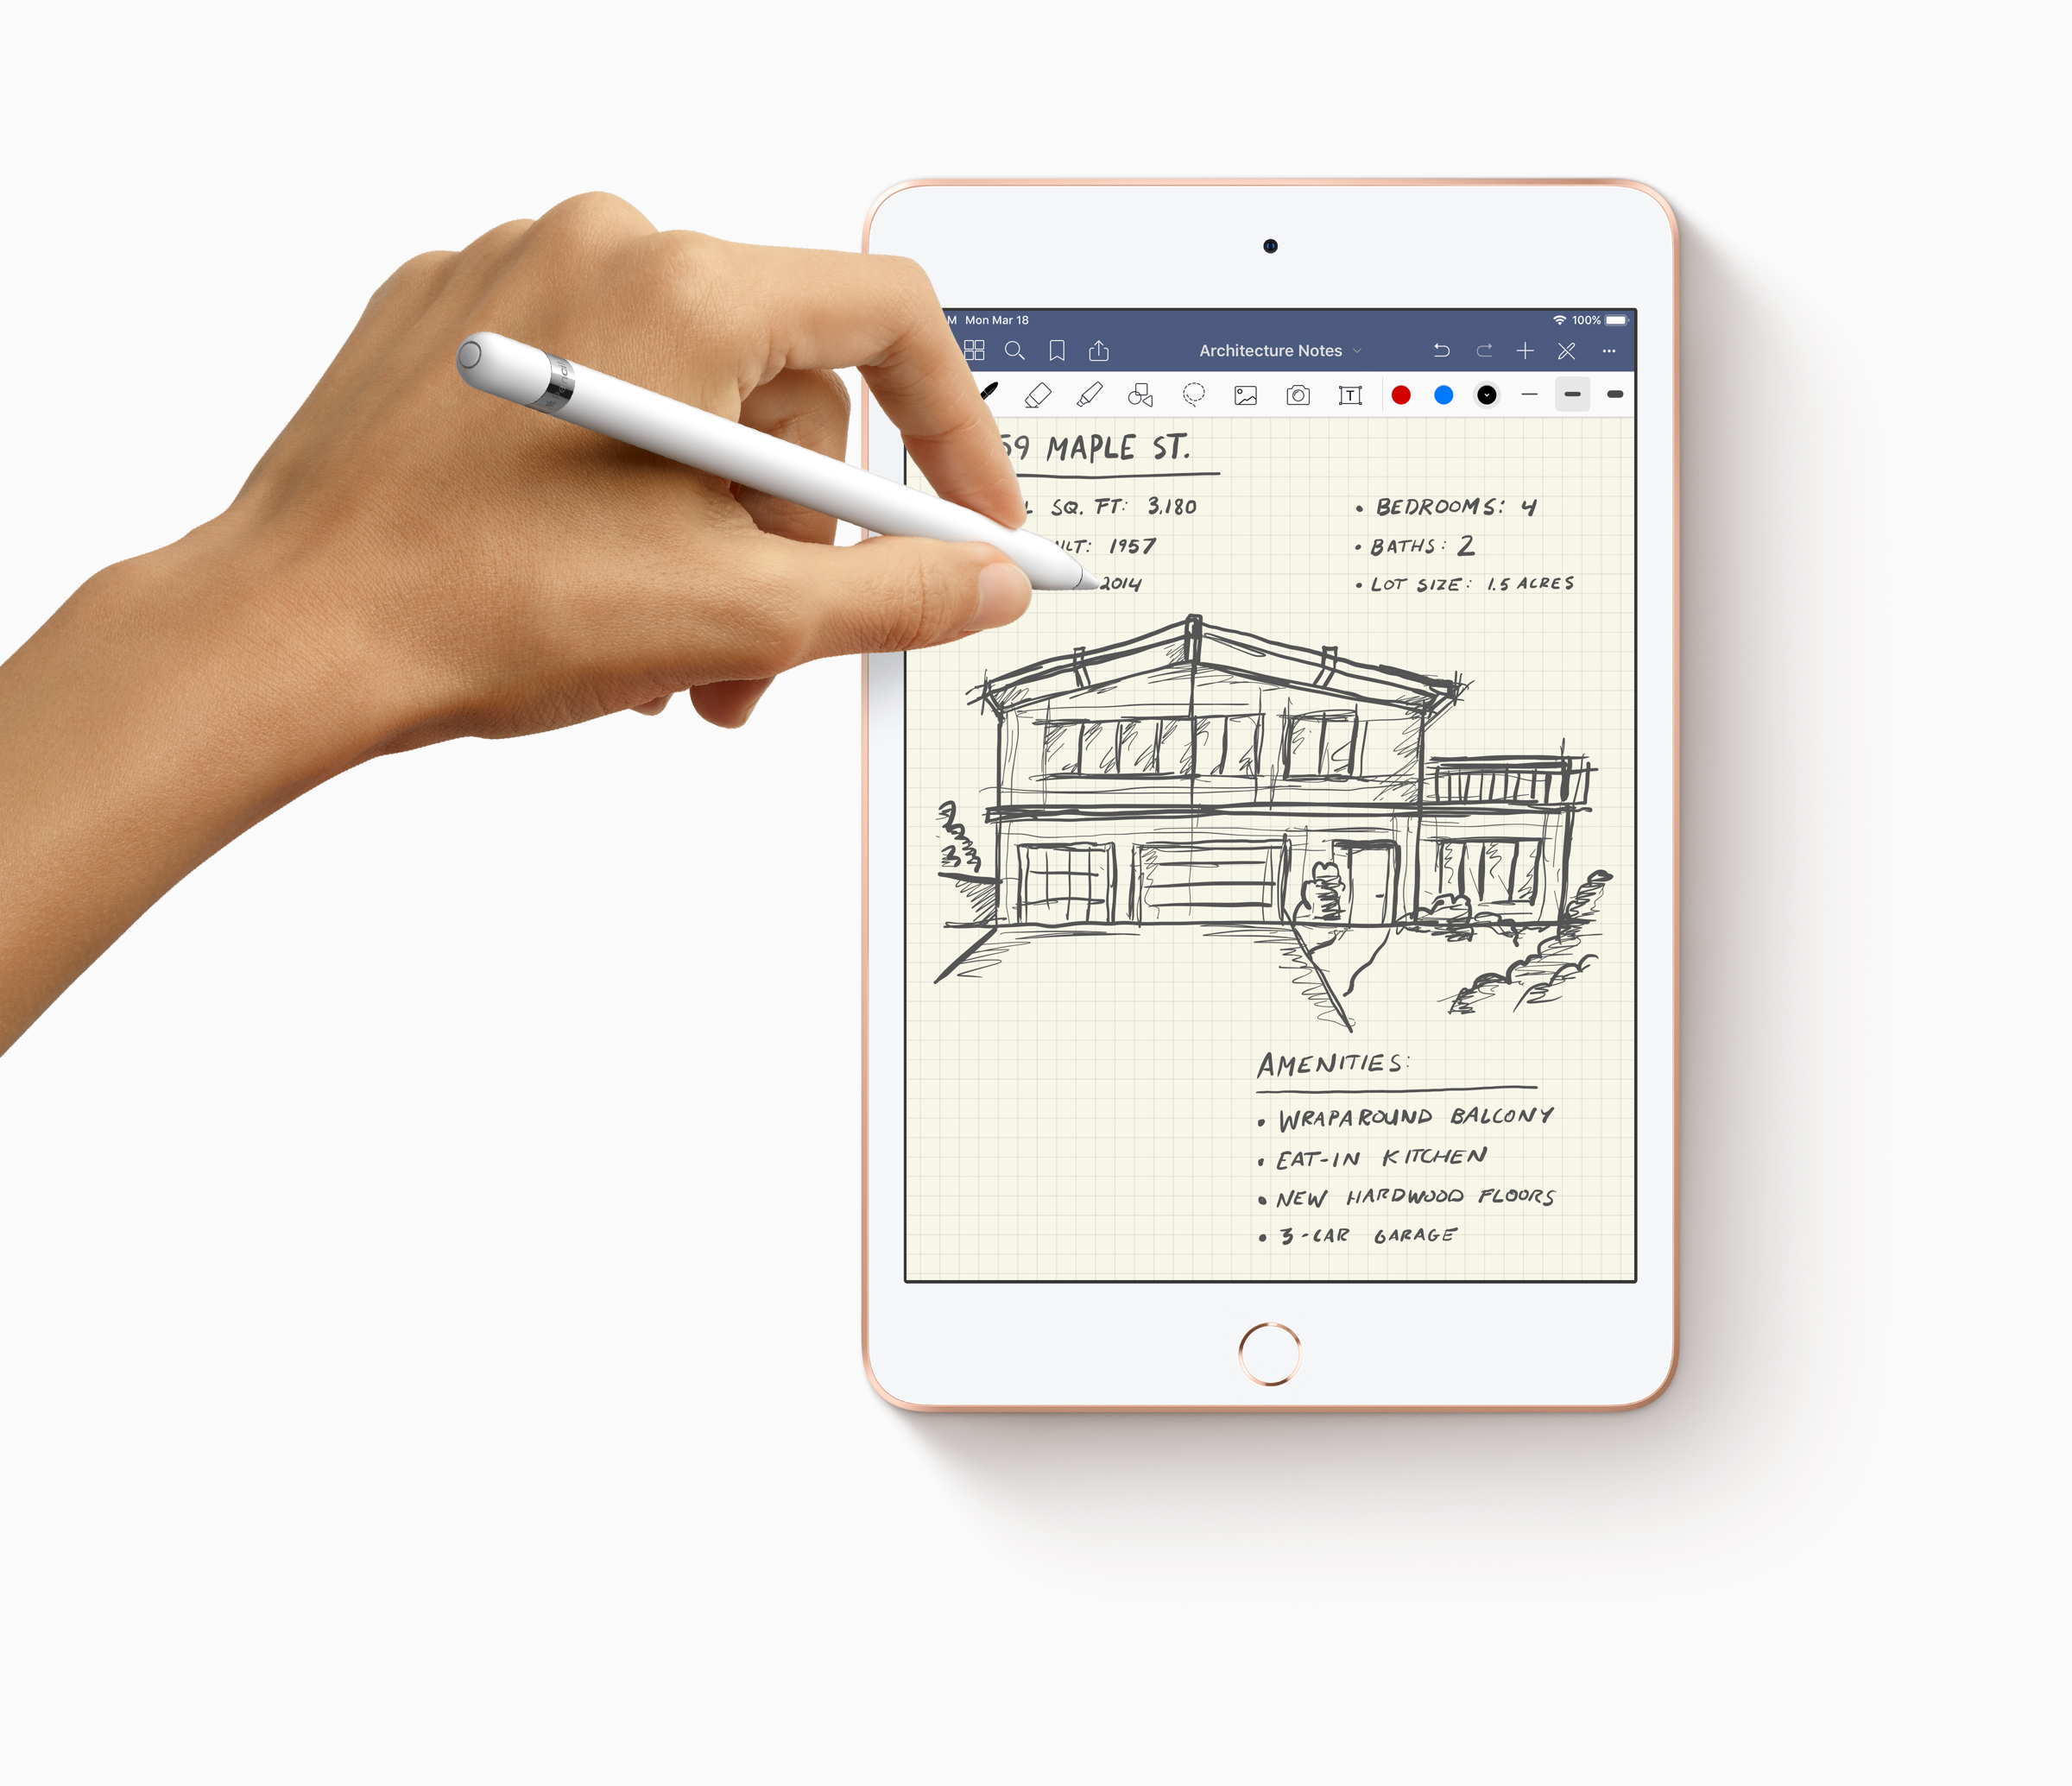
\includegraphics[width=60mm]{images/ipadmini.jpg}}
                         \end{center} \caption{Apple iPad} \label{fig:ipad}
\end{minipage} \begin{minipage}{0.5\hsize}
                   \begin{center} \fbox {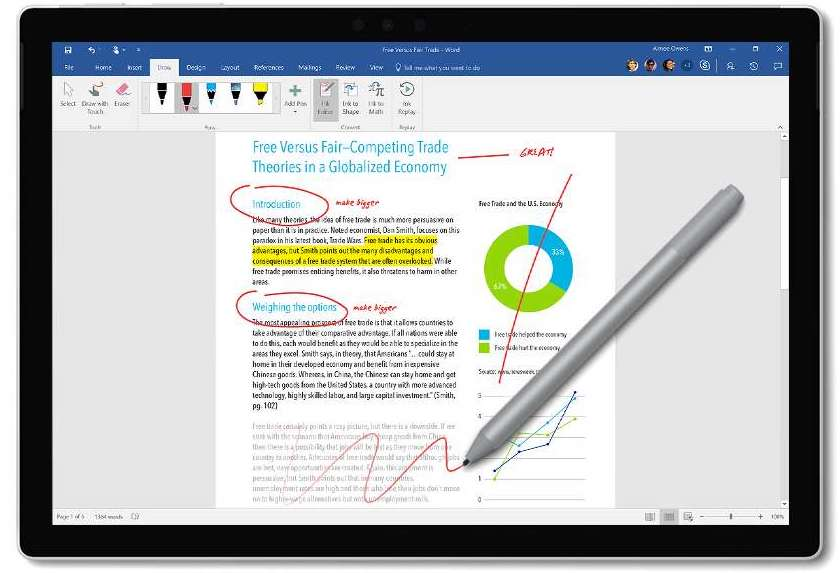
\includegraphics[width=60mm]{images/surface.jpg}}
                   \end{center} \caption{Microsoft Surface} \label{fig:surface}
\end{minipage}
\end{figure}


\section{手書きメモ・イラストの現状}
計算機上で手書きメモ・イラストを扱う主要なシステムを紹介し、計算機における手書きメモの現状を解説する。

\subsection{iOSのメモアプリ}

\begin{figure}[htbp]
    \begin{center}
        %        \fbox {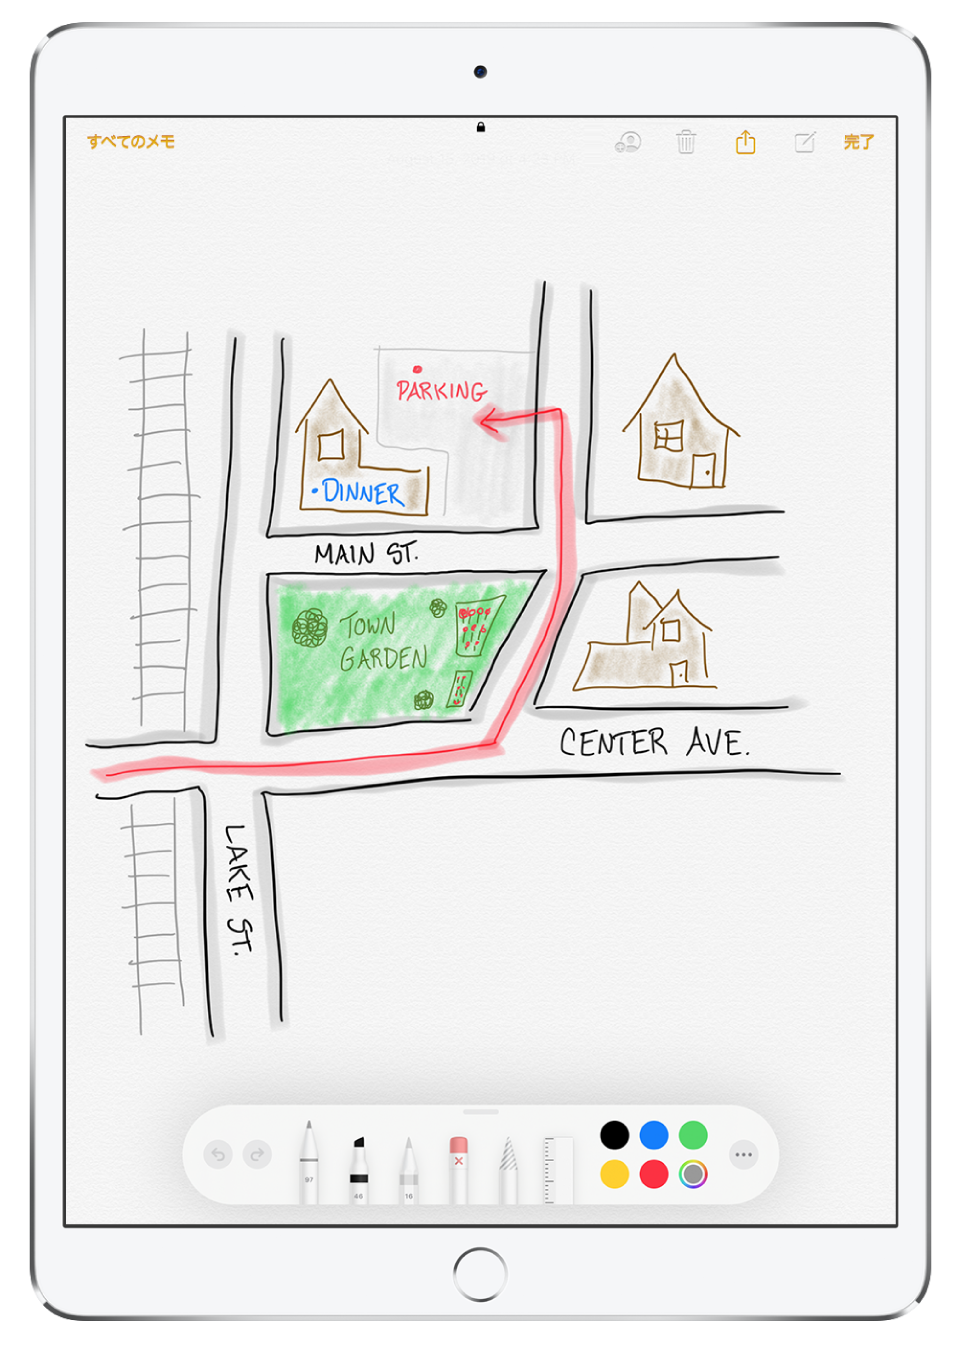
\includegraphics[width=50mm]{images/applememo.png}} \end{center}
        \fbox {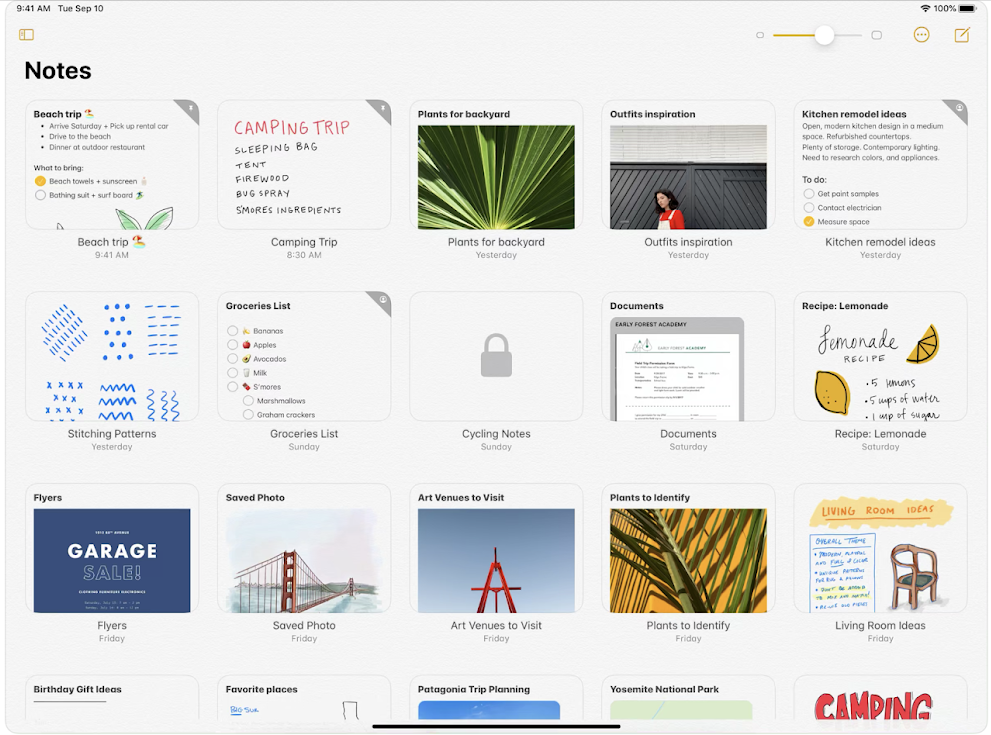
\includegraphics[width=100mm]{images/iosmemo.png}} \end{center}
    \caption{iOSのメモアプリ} \label{fig:iosmemo}
\end{figure}

Apple\footnote{https://www.apple.com/}のiOSデバイスにはメモアプリケーションが標準でインストールされており、指やApple Pencilを用いて素早く手書きメモを取ることができる。
一方で描いた手書きメモは単なる画像として扱われ、それを後から検索する機能は存在しないため 作成した手書きメモを参照可能な状態にするには
ルールに基づいてファイル名を決めたり、図\ref{fig:iosmemo}のようにフォルダに分類して保存する等の工夫が求められる。

\subsection{Evernote}

\begin{figure}[htbp]
    \begin{center}
        \fbox {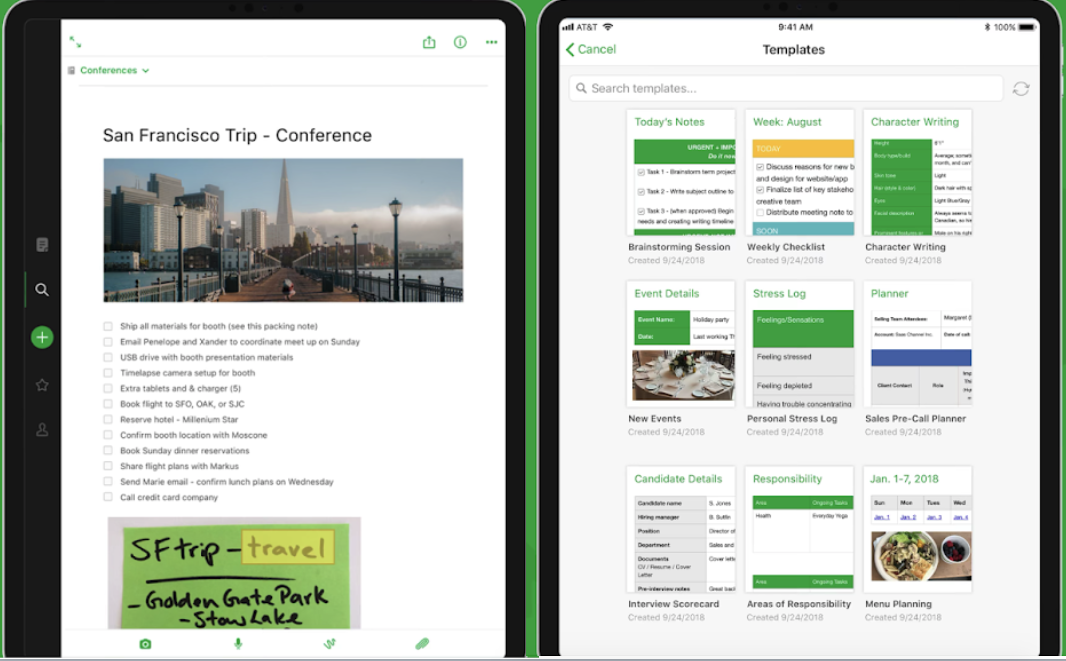
\includegraphics[width=100mm]{images/margedevernote.png}} \end{center}
    \caption{Evernote} \label{evernote} \label{fig:evernote}
\end{figure}

Evernote Corporation\footnote{https://evernote.com/intl/jp/about}が開発するEvernote(図\ref{fig:evernote})も指やスタイラスペンによって手書きのメモやスケッチを作成できる。
またiOS標準のメモアプリと同様にノートブックと呼ばれる分類用のフォルダを備えるほか、ラベルによってメモを分類することもできる。
さらに手書きメモ内の文字を認識し、全文検索によって手書きメモを検索する機能を備えているが、
検索対象は認識できた手書き文字のみであり、図形や描いたものの形状等のグラフィカルなデータから手書きメモを検索することはできない。
\\
\\
またいずれのメモアプリケーションも、作成した手書きのメモをそのアプリケーション以外のシステムで再利用することが難しく、相互運用性に問題がある。
例えば作成したiOSのメモアプリやEvernoteで作成した手書きメモをWebサイトに埋めこむことはできない。いずれのアプリも手書きの部分を
独立した画像ファイルとして出力できるが、その場合はメモに関するフォルダやラベル等の分類情報も欠落してしまう。


\section{手書きメモ・イラストの問題点}
\label{mondai}
現状の手書きメモ・イラストが抱える問題点を整理する。
\begin{enumerate}
    \item 検索ができないため参照や管理が面倒\\
    テキストと異なり手書きメモ・イラストはそのものを検索することができないため参照しづらい。
    参照可能な状態にしておくためにはフォルダやラベルによる分類等の管理が必要とされる。
    \item 再利用が難しい\\
    Webサイトへの埋め込み等、作成したメモアプリケーション以外で手書きメモを再利用することが難しい。
\end{enumerate}

\section{テキストの進化}
手書きに先んじて計算機上で利用されているテキストは、文字から内容を検索することが可能なため
文書の参照や管理が格段に行いやすく、あらゆる文書の作成やメール等の連絡手段が電子化されたテキストに置き換えられるようになった。
またWebやハイパーリンク等の技術によってより参照しやすくなったほか、別の文書を引用する等の再利用が可能になった。
さらにハイパーリンクを含んだ文書(ハイパーテキスト)を手軽に作成・編集できるWiki\cite{Leuf2001TheWW}が登場したことで
より柔軟かつ活発なテキストによる知見の共有や情報の再利用が実現された。

\subsection{Scrapbox}
Wikiシステムの例としてGyazz\cite{Gyazz}をベースに開発され、Nota\footnote{\textsf{https://www.notainc.com/ja}}社よって運営されている
Scrapbox\footnote{http://scrapbox.io/}を挙げる(図\ref{fig:scrapbox1})。
Scrapboxは\texttt{[]}を基本としたシンプルな記法とWYSIWYGエディタによって
ページ間のリンクや外部リンクを含んだ画像や動画を簡単に記述することができる。
また図\ref{fig:scrapbox2}のようにページの下部に
\begin{itemize}
    \item 別ページへのリンク
    \item 別ページからのリンク
    \item リンク先ページがリンクしているページ
\end{itemize}等のリンク情報に基づいた関連ページを推薦し表示する機能を備えている。
Scrapboxには分類用のフォルダ等の機能は存在せず全てのページがフラットに管理されるが、
リンクによって関連するページが自動的に分類されるため管理のための特別な工夫を必要とせずに
多数のページを運用することができる。

このようにWikiシステムによって文書の参照や管理が容易になり、さらなる情報の再利用が可能になった。

\begin{figure}[htbp] \begin{minipage}{0.5\hsize}
                         \begin{center} \fbox{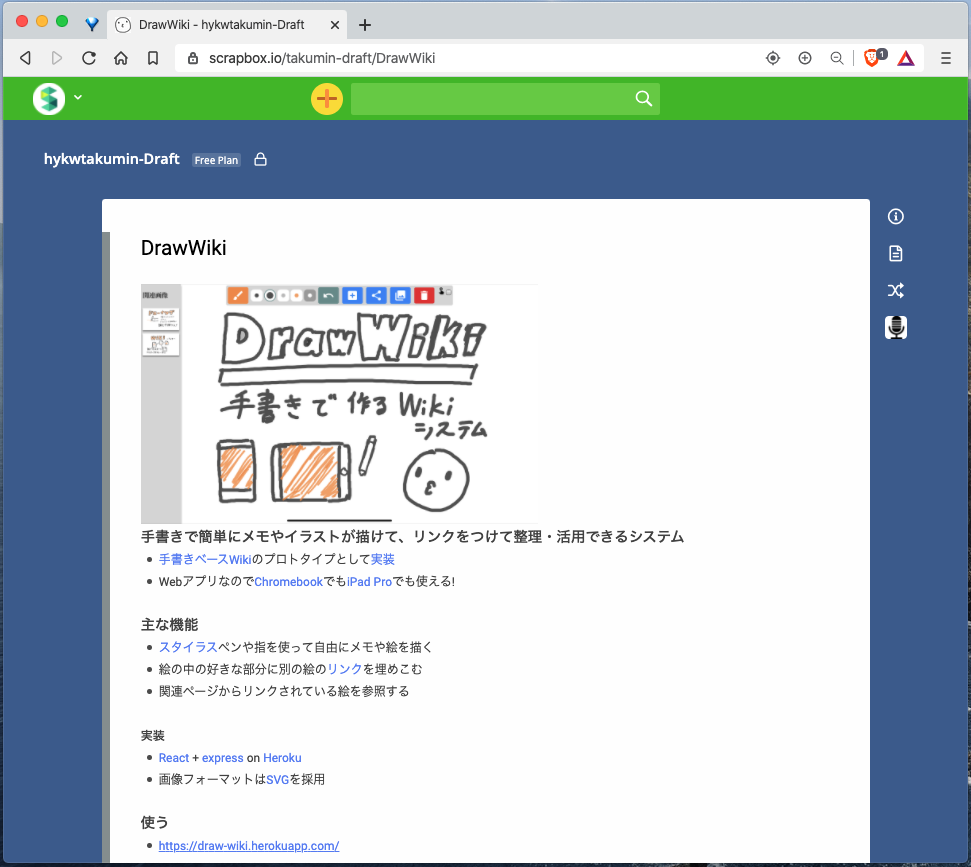
\includegraphics[width=70mm]{images/scrapbox1.png}}
                         \end{center} \caption{Scrapboxの画面} \label{fig:scrapbox1}
\end{minipage} \begin{minipage}{0.5\hsize}
                   \begin{center} \fbox{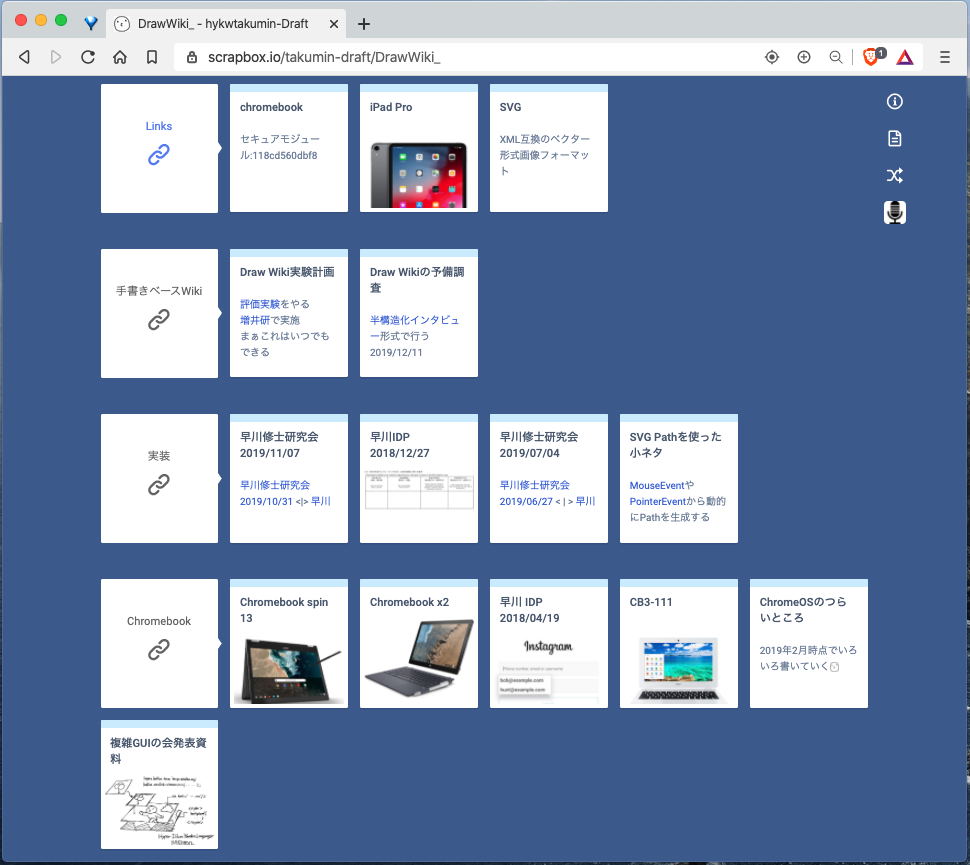
\includegraphics[width=70mm]{images/scrapbox2.png}}
                   \end{center} \caption{関連ページリスト} \label{fig:scrapbox2}
\end{minipage}
\end{figure}


\section{まとめ}
手書きメモ・イラストは広く浸透した情報の記録・表現手法であるものの、参照や管理には問題があり、再利用も制限されている。
一方でテキストは計算機上でも積極的に応用されており、Wiki等の技術によって文書の参照や管理が容易になったことからさらなる
情報の再利用が実現された。したがって同様の技術を手書きメモ・イラストに適用することができれば、問題を解決できると考えられる。
次章では手書きメモをハイパーテキストとして扱い、Wikiのように運用できるシステム「手書きベースWiki」を提案し、その設計について述べる。

%\section{まとめ}
%手書きメモ・イラストは広く浸透した情報の記録手法であるものの、紙というフォーマットの制約によって使い勝手が制限されている。
%一方で計算機上で手書きメモ・イラストの作成や管理を行うシステムが広く利用されているが、画像ファイルフォーマットの制約から
%これらは紙の手書きメモの利用形態を再現したにとどまり、参照や管理、再利用が難しいという本質的な問題は解決されていない。
%次章では上記のような問題点を解決するべく、これまでの手書きメモ・イラストの在り方にとらわれない次世代のフォーマット「ハイパーイラスト」と、
%それらを容易に管理・再利用できるシステム「手書きベースWiki」を提案する。